\section{Zitierformate}
\label{sec:zitierformate}
In der Wissenschaft gibt es viele verschiedene Zitierweisen, die sich je nach Fachgebiet unterscheiden.
In dieser Arbeit soll jedoch nicht auf die verschiedenen Zitierweisen eingegangen werden, sondern auf Zitierformate, welche für die Zitation verwendet werden können und die Datenstruktur hinter der Zitation beschreiben.
Hierbei gibt es ebenfalls unterschiedliche Formate, wobei sich in dieser Arbeit auf das \gls{cff} und das \hologo{BibTeX}-Format beschränkt werden.
Das \gls{cff} ist ein Format, welches speziell für die Zitation von Software entwickelt wurde, weshalb es in dieser Arbeit besonders interessant ist.
Das \hologo{BibTeX}-Format wird dazu verwendet, um zumeist in Verbindung mit \LaTeX{} Bibliographien zu erstellen und ist daher ebenfalls von Interesse, da es auch für Software verwendet werden kann und von vielen eingesetzt wird.

\subsection{Citation File Format}
\label{subsec:citation-file-format}
Das \gls{cff} ist ein Format, welches in der Datei \mintinline{text}{CITATION.cff} gespeichert wird und in YAML 1.2 geschrieben wird. 
Das Format beschreibt die Zitation von Software und kann von Menschen und Maschinen gelesen werden.
Es enthält Metadaten, welche für die Zitation von Software benötigt werden.
Außerdem wird es öffentlich auf GitHub verwaltet.
Softwareentwickler können das \gls{cff} in ihre Repositorys einbinden, um anderen die Zitation ihrer Software zu erleichtern und vorzugeben, wie die Software richtig zu zitieren ist \autocite{druskat_citation_2021}.

Da die Datei von Menschen gelesen werden kann, kann diese manuell erstellt werden und in das Repository eingebunden werden.
Die Spezifikationen für das \gls{cff} werden auf GitHub verwaltet und sind öffentlich einsehbar \autocite{druskat_citation_2021}.
Ebenfalls existieren Programme, welche das \gls{cff} verarbeiten können.
Beispielsweise kann das Programm \emph{cffinit} genutzt werden, um eine \mintinline{text}{CITATION.cff}-Datei zu erstellen, sodass der Prozess der Erstellung vereinfacht wird \autocite{spaaks_cffinit_2023}.
Ein weiteres Beispiel ist das Programm \textit{cffconvert}, welches das \gls{cff} in verschiedene Formate umwandeln kann, wie zum Beispiel \hologo{BibTeX} oder RIS \autocite{spaaks_cffconvert_2021}.

Zusätzlich wird das \gls{cff} von unterschiedlichen Plattformen unterstützt, wie zum Beispiel von GitHub.
Erkennt GitHub eine \mintinline{text}{CITATION.cff}-Datei im Repository auf dem Standardbranch, wird sie automatisch auf der Repository-Startseite verlinkt und kann direkt im \hologo{BibTeX}-Format kopiert werden \autocites{druskat_citation_2021}{github_about_2024-2}.
Ebenfalls ist es möglich die in der Datei eingetragenen Autoren in der APA-Zitierweise zu kopieren.
Die Funktionen sind in \autoref{fig:gh_cff_link} dargestellt.
Eine weitere Plattform, welche unterstützt wird, ist Zotero, welches ein Literaturverwaltungsprogramm ist \autocites{druskat_citation_2021}{zotero_zotero_2024}.
Falls der Benutzer das Browser-Plugin von Zotero installiert hat, liest dieses die Daten aus der \mintinline{text}{CITATION.cff}-Datei, welche in dem GitHub Repository gespeichert ist und importiert die Daten in Zotero.

\begin{figure}
    \centering
    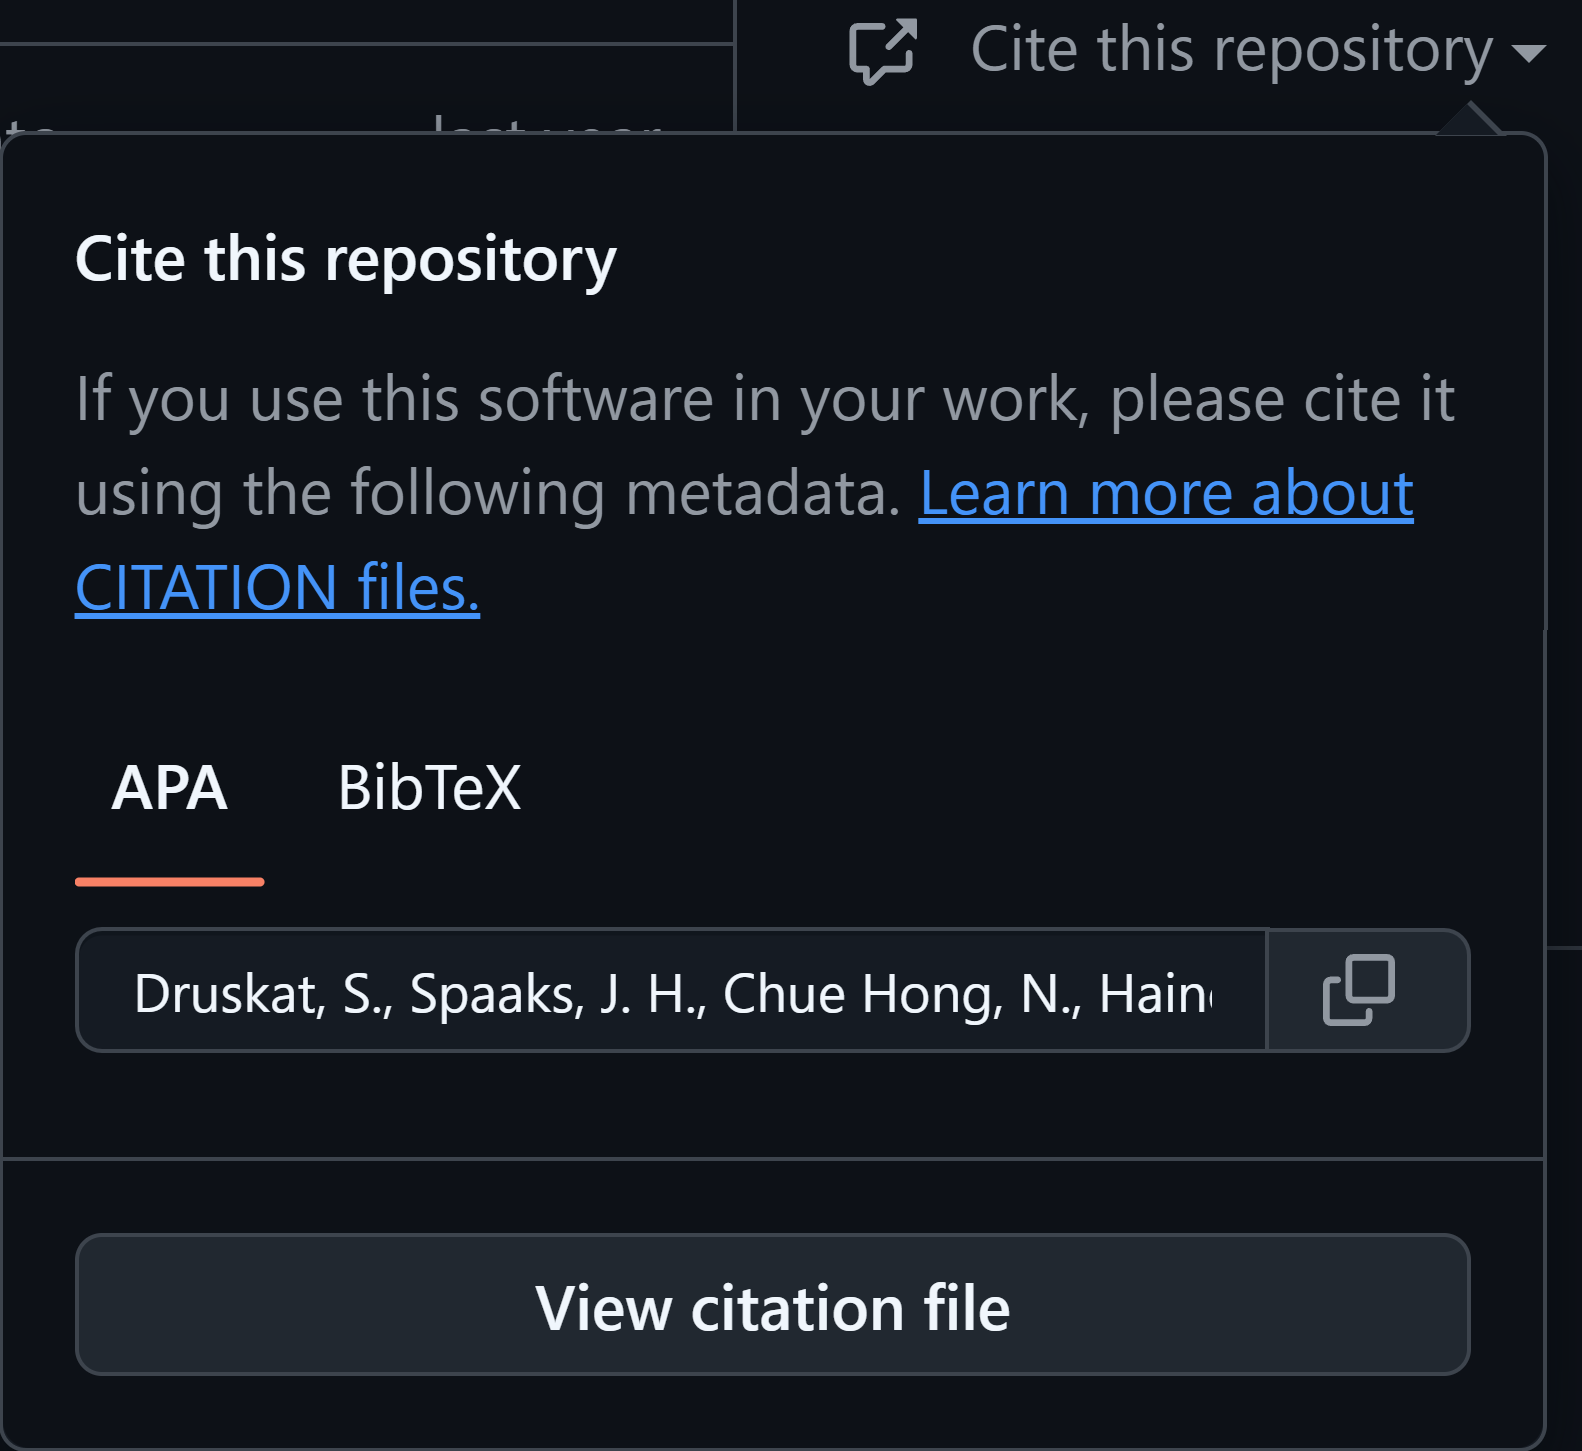
\includegraphics[width=0.5\textwidth]{bilder/GH_CFF_link.png}
    \caption{GitHub-Repository mit \mintinline{text}{CITATION.cff}-Datei}
    \label{fig:gh_cff_link}
    \small
    Die Abbildung stellt den Link auf die \mintinline{text}{CITATION.cff}-Datei dar, wie ihn GitHub aktuell darstellt.
    Außerdem ist die Möglichkeit sichtbar, die Datei im \hologo{BibTeX}-Format und in der APA-Zitierweise zu kopieren.
\end{figure}

In dem \gls{cff} existieren verschiedene Felder, welche für die Zitation von Software relevant sind.
In dieser Masterarbeit wird auf einige dieser Felder eingegangen, welche für die spätere Auswertung relevant sind.
Das wichtigste Feld ist das \glqq authors\grqq{}-Feld, welches die Autoren der Software enthält und zwingend erforderlich ist.
In diesem Feld können die Autoren als Liste angegeben werden.
Ein Autor ist dabei entweder eine Person oder eine Entität.
Eine Entität kann beispielsweise eine Organisation oder ein Unternehmen sein.
Die Entität kann mit einem Namen mittels \glqq name\grqq{} angegeben werden \autocite{druskat_citation_2021}.
Sie kann ebenfalls eine ORCID iD und eine E-Mail-Adresse enthalten.
Besonders wichtig für diese Arbeit ist die Referenz auf eine Person, da dies die einzige Information ist, welche aus Git extrahiert werden kann.
Eine Person enthält ebenfalls die genannten Werte einer Entität und wird jedoch über den Vor- und Nachname separiert mittels \glqq given-names\grqq{} und \glqq family-names\grqq{} angegeben.
Dadurch ist es möglich die Personen von den Entitäten zu unterscheiden.

Ein weiteres Feld, welches in der Masterarbeit relevant ist, ist das \glqq preferred-citation\grqq{}-Feld.
Mit diesem Feld ist es möglich die Anerkennung für die Arbeit auf eine andere Arbeit zu übertragen \autocite{druskat_citation_2021}.
Ein Beispiel hierfür ist ein Paper über die Software, welches bevorzugt zitiert werden soll anstelle der eigentlichen Software.
Hierbei können ebenfalls Personen und Entitäten angegeben werden in dem gleichen Format wie bereits beschrieben.
Durch die Angabe einer \glqq preferred-citation\grqq{} kann das Prinzip der Wichtigkeit vernachlässigt werden.
Auf dieses Verhalten wird in den Ergebnissen konkreter eingegangen.

Weitere in der Arbeit verwendete Felder sind \glqq type\grqq{}, \glqq year\grqq{}, \glqq month\grqq{}, \glqq date-released\grqq{} und \glqq date-published\grqq{} \autocite{druskat_citation_2021}.
Das Feld \glqq type\grqq{} ist zwingend erforderlich, hat jedoch als Standardwert \glqq software\grqq{}, sodass dies nicht angegeben werden muss.
Das Feld gibt an, ob es sich um eine Software oder einen Datensatz handelt.
Falls das Feld unter dem Feld \glqq preferred-citation\grqq{} angegeben wird, kann es viele weitere Typen enthalten wie Beispielsweise \glqq thesis\grqq{} oder \glqq manual\grqq{}, sodass diese Arbeiten ebenfalls referenziert werden können.
Das Feld \glqq date-released\grqq{} gibt an, wann die Software oder der Datensatz veröffentlicht wurde.
Die Felder \glqq year\grqq{}, \glqq month\grqq{} und \glqq date-published\grqq{} können zusätzlich zu dem Feld \glqq date-released\grqq{} unter dem Feld \glqq preferred-citation\grqq{} angegeben werden, um das Jahr und das Datum der Veröffentlichung anzugeben.
Ein Beispiel einer \mintinline{text}{CITATION.cff}-Datei ist in \autoref{lst:cff_example} dargestellt.
Dabei sind wurde sich auf die beschriebenen und notwendigen Felder beschränkt.

% TODO Update date with my actual date
\begin{listing}
    \inputminted{yaml}{../CITATION.cff}
    \caption{Beispiel einer \mintinline{text}{CITATION.cff}-Datei}
    \label{lst:cff_example}
\end{listing}

\subsection{\hologo{BibTeX}}
\label{subsec:bibtex_format}
\hologo{BibTeX} ist eine Software, welche zur Erstellung von Literaturangaben und -verzeichnissen in \LaTeX{}-Dokumenten verwendet wird.
Außerdem existiert mit \hologo{BibTeX} ein gleichnamiges Format, welches in der Datei \mintinline{text}{CITATION.bib} gespeichert wird und auf keinem anderen Format basiert.
\hologo{BibTeX} ist ein weit verbreiteter Standard und wird von vielen verwendet, um Literatur zu zitieren. % TODO ggf. finde ich hier noch genaue zahlen? -> ist immer ganz nett sowas zu haben
Das Format beschreibt die Zitation von Literatur und kann von Menschen und Maschinen gelesen werden.
Es beschränkt sich dabei nicht auf eine spezielle Art von Literatur, sondern kann für viele unterschiedliche Arten von Literatur verwendet werden.
Beispielsweise können Bücher und Masterarbeiten in \hologo{BibTeX} zitiert werden \autocite{patashnik_bibtexing_1988}.
Ein offizieller Literaturtyp für Software existiert nicht.
In der Datei können mehrere Einträge vorhanden sein, wobei jeder Eintrag eine Literaturangabe darstellt.

\hologo{BibTeX}-Dateien können von Menschen manuell erstellt werden und in das Repository eingebunden werden.
Außerdem existieren viele Literaturverwaltungsprogramme wie Zotero, welche \hologo{BibTeX}-Dateien erstellen und verarbeiten können \autocite{zotero_zotero_2024}.
Ebenfalls ist die Integration in andere Plattformen möglich, wie zum Beispiel in GitHub.
Hier wird die \mintinline{text}{CITATION.bib}-Datei auf der Repository-Startseite verlinkt, sie lässt sich jedoch im Gegensatz zu dem \gls{cff} nicht direkt kopieren oder in andere Formate umwandeln \autocite{github_about_2024-2}.

In dem \hologo{BibTeX}-Format existieren verschiedene Felder, welche für die Zitation von Literatur relevant sind.
Einige Felder sind dabei zwingend erforderlich und andere nicht.
Welche Felder zwingend erforderlich sind, hängt vom Literaturtyp ab.
Außerdem sind die verfügbaren Felder vom Literaturtyp abhängig \autocite{patashnik_bibtexing_1988}.
In dieser Arbeit wird auf einige dieser Felder eingegangen, welche für die spätere Auswertung relevant sind.
Das wichtigste Feld ist das \glqq author\grqq{}-Feld, welches die Autoren der Literatur enthält und zwingend erforderlich ist.
Die Vor- und Nachnamen der Autoren werden mit einem Komma separiert und mehrere Autoren über ein \glqq and\grqq{} getrennt.
Weitere Felder, welche für die Masterarbeit verwendet werden, sind \glqq year\grqq{} und \glqq month\grqq{}, welche das Jahr und den Monat der Veröffentlichung angeben.
Ein Beispiel einer \mintinline{text}{CITATION.bib}-Datei ist in \autoref{lst:bibtex_example} dargestellt.
Es ist zu erkennen, dass in dem \hologo{BibTeX}-Eintrag Informationen fehlen, welche in dem \gls{cff}-Eintrag vorhanden waren.
Dies liegt daran, dass in dem \hologo{BibTeX}-Eintrag nur eine Referenz auf die Masterarbeit möglich ist und nicht auf die entwickelte Software.

% TODO Update date with my actual date
\begin{listing}
  \inputminted{text}{../CITATION.bib}
  \caption{Beispiel einer \mintinline{text}{CITATION.bib}-Datei}
  \label{lst:bibtex_example}
\end{listing}
